\documentclass{beamer} 
\usetheme{Singapore} 

%\setbeameroption{show notes}

\usepackage{color}
\usepackage{amsmath}


\title{Bayesian Inference for Arts Majors}
\author{Marius Cobzarenco}
\date{December 2012}

\begin{document}
	\maketitle
	\begin{frame}

		\frametitle{Two Schools of Thought}
		\begin{itemize}
			\item What is probability?
			\pause
			\item People have an innate understanding of uncertainty
			\pause
			\item E.g. natural languages make it easy to describe and assign likelihoods to different outcomes of a situation.
			\pause
			\item However, formalizing this intuition into maths turns out to be a bit tricky.
			\pause
			\item Consider two questions:
			\begin{enumerate}
				\item What's the probability of getting heads if you flip a coin?
				\pause
				\item What's the probability that alien life exists in the universe?
			\end{enumerate}
			\pause
			\item Historically, this distinction has lead to two opposing philosophical views of probability.
		\end{itemize}

	\end{frame}
	\note {
	\begin{itemize}
		\item The obligatory over-used stats metaphor
		\item The question "What's the probability of getting heads if a flip a coin?" is not so different as it is possible to calculate the outcome.
\item Well, maybe we can flip coins for long enough and average the results and thus probability = \emph{long term average}.
	\end{itemize}
	}

	\begin{frame}
		\frametitle{Frequentist Probability}
		\begin{columns}
			\begin{column}{0.4\textwidth}
				\begin{figure}
					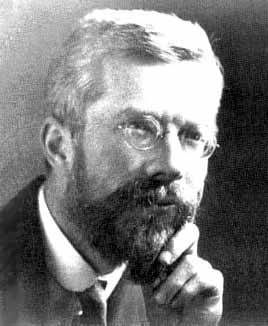
\includegraphics[scale=0.53]{fischer.jpg}
					\begin{centering}
						\small Ronald Fisher (1890 -- 1962)
					\end{centering}
				\end{figure}
			\end{column}	

			\begin{column}{0.6\textwidth}
				\begin{itemize}
					\item Probability = long term average over (hypothetical) repeated experiments.
					\pause
					\item Data is random
					\pause
					\item Quantities of interest (i.e. the parameters)  are not random, only unknown.
					\pause
					\item The \emph{sampling distribution} is of central importance.
					\pause
					\item "Standard" interpretation of probability.
				\end{itemize}
			\end{column}
		\end{columns}
	\end{frame}
	\note {
	\begin{itemize}
		\item the idea of repeated experiments is central (hence the name "freqentist")
		\item central concept: The sampling distribution of a statistic is the distribution of that statistic, considered as a random variable, when derived from a random sample of size n. 
		\item The sampling distribution depends on the underlying distribution of the population, the statistic being considered, the sampling procedure employed and the sample size used. There is often considerable interest in whether the sampling distribution can be approximated by an asymptotic distribution, which corresponds to the limiting case as n → ∞.

	\end{itemize}
	}

	\begin{frame}
		\frametitle{Bayesian Probability}
		\begin{columns}
			\begin{column}{0.4\textwidth}
					\begin{figure}
					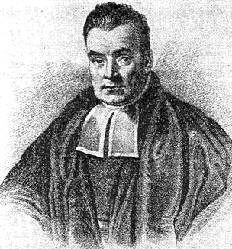
\includegraphics[scale=0.53]{bayes.jpg}
					\begin{centering}
						{\small Thomas Bayes (1701 -- 1761)}
					\end{centering}
				\end{figure}
			\end{column}	

		\begin{column}{0.6\textwidth}
			\begin{itemize}
				\item Probability is subjective, $P(A) \equiv \text{how likely we think A is true}$
				\pause
				\item Probability $\equiv$ strength of belief
				\pause
				\item Hence one can consistently use probabilities in any uncertain situation.
				\pause 
				\item Maintains a distribution over the quantities of interest.
				\pause 
				\item Bayes theorem used for inference.

 			\end{itemize}
		\end{column}
	\end{columns}
		
	\end{frame}

	\note {
	\begin{itemize}
		\item "subjective" probability
		\item 

	\end{itemize}
	}

	\begin{frame}
		\frametitle{Also... Bayes is back}
		\begin{columns}
			\begin{column}{0.4\textwidth}
				\begin{figure}
					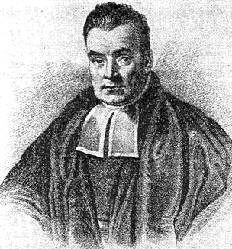
\includegraphics[scale=0.53]{bayes.jpg}
					\begin{centering}
						{\small Thomas Bayes (1701 -- 1761)} 
					\end{centering}
				\end{figure}
			\end{column}	
			\begin{column}{0.6\textwidth}
				\begin{figure}
					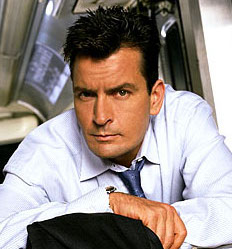
\includegraphics[scale=2.4]{newbayes.jpg}
				\end{figure}
			\end{column}	
\end{columns}

	\end{frame}

	\begin{frame}
		\frametitle{Bayes Theorem}
		\begin{itemize}
			\pause
			\item A bit of notation: $P(A|B)$ reads "the probability of A given B" 
			\pause
			\item E.g. the probability of being ill given that my doctor told me so
			\pause
			\item Or closer to finance, e.g.: the probability of making a profit if I put all my money on red
			\pause
			\item Bayes Theorem gives a way of updating beliefs when confronted with evidence:
			\begin{displaymath}
			P(A|B) = \frac{P(B|A)P(A)}{P(B)}
			\end{displaymath}
			\pause
			\item The workhorse of Bayesian inference, used to compute $P(\text{what I care about} | \text{what I have observed})$.
			\pause
			\item It also fits on a t-shirt
		\end{itemize}
	
	\end{frame}

	\note {
		\begin{itemize}
			\item e.g. the probability of being ill given that my doctor told me so
			\item or for an example closer to finance: the probability of making a profit if I put all my money on red
			\item If you need ideas for Chirstmas presents
		\end{itemize}
	}

	\begin{frame}
		\frametitle{A Medical Example}
		\begin{quote}
			1\% of women at age forty who participate in routine screening have breast cancer.  80\% of women with breast cancer will get positive mammographies.  9.6\% of women without breast cancer will also get positive mammographies. 
	\end{quote}
	\begin{quote}
 A woman in this age group had a positive mammography in a routine screening.  What is the probability that she actually has breast cancer?
		\end{quote}
		\pause
		Formalizing, we want to know $P(\text{cancer} |\text{positive})$
		\pause
		\begin{enumerate}
			\item $>$ 70\%
			\item 30\% -- 70\%
			\item $<$ 30\%
		\end{enumerate}
	\end{frame}

	\note{
		ask them to guess the answer
	}

	\begin{frame}
		\frametitle{A Medical Example (cont.)}
		\begin{quote}
			1\% of women at age forty who participate in routine screening have breast cancer.  80\% of women with breast cancer will get positive mammographies.  9.6\% of women without breast cancer will also get positive mammographies. 
		\end{quote}
		\begin{displaymath}
			P(\text{cancer} |\text{positive})=\frac{P(\text{positive} |				\text{cancer})P(\text{cancer})}{P(\text{positive})}
		\end{displaymath}
		\pause
		\begin{align*}
		P(\text{cancer}) &= 1\% \\
		P(\text{positive} |\text{cancer}) &= 80\% \\
		P(\text{positive}) &= P(\text{positive}|\text{cancer})P(\text{cancer}) + \\
			&\quad P(\text{positive}|\text{no cancer})P(\text{no cancer}) \\
			&= 80\% \times 1\% + 9.6\% \times 99\% = 10.3\%
		\end{align*}
	\end{frame}

	\begin{frame}
		\frametitle{A Medical Example (cont.)}
		\begin{displaymath}
		P(\text{cancer}) = 1\%,\quad P(\text{positive} |\text{cancer}) = 80\%, \quad
		P(\text{positive}) = 10.3\%
		\end{displaymath}
		\pause
		\begin{align*}
			P(\text{cancer} |\text{positive})&=\frac{P(\text{positive} |				\text{cancer})P(\text{cancer})}{P(\text{positive})}\\
				&= \frac{80 \% \times 1\%}{10.3 \%} = 7.77 \%
		\end{align*}
		\pause
		Studies suggest that most doctors estimate the probability to be between 70\% and 80\% (wildly incorrect). [Casscells, Schoenberger, and Grayboys 1978; Eddy 1982; Gigerenzer and Hoffrage 1995]
	\end{frame}

	\note {
	Next, suppose I told you that most doctors get the same wrong answer on this problem - usually, only around 15\% of doctors get it right.  ("Really?  15\%?  Is that a real number, or an urban legend based on an Internet poll?"  It's a real number.  See Casscells, Schoenberger, and Grayboys 1978; Eddy 1982; Gigerenzer and Hoffrage 1995; and many other studies.  It's a surprising result which is easy to replicate, so it's been extensively replicated.)
	}

	\begin{frame}
		\frametitle{A Financial Example}
		\begin{itemize}
			\item My broker sends me a trade idea every day and I'd like to estimate their hit rate.
			\pause
			\item  Bayes Theorem induces a distribution over different possible values of the hit rate:
			\pause
			\item []
			\begin{displaymath}
				P(\text{rate} |\text{trade ideas})=\frac{P(\text{trade ideas} |				\text{rate})P(\text{rate})}{P(\text{trade ideas})}
			\end{displaymath}
			\pause
			\item Even better, we can apply it iteratively:
			\begin{align*}
				P(\text{rate} |\text{trade ideas})=\frac{P(\text{idea} |					\text{rate}, \text{prev. ideas})P(\text{rate} | \text{prev. ideas})}{P(\text{trade ideas})}
			\end{align*}
		\end{itemize}

	\end{frame}
	\note {
		\begin{itemize}
		\item {The obvious frequentist estimate is the number of ideas with positive returns divided by the total number of trade ideas}
		\item Talk about what happens when there are just a few ideas and how the Bayesian framework avoids over-fitting in a principled manner.
		\item Talk about treating parameters as a random variable rather than an unknown parameter.
		\item Talk more about priors
		\item Built in Occam's razor
		\end{itemize}
	}
		


\input{hitrate.tex}

\end{document}